\section{Finding Shapes}

\subsection{Thresholding and Subtraction}

\subsubsection{Thresholding}
We can use thresholding for basic feature extraction, if the shape to be extracted is defined by its brightness. However we do not obtain the full shape from thresholding if the intensity levels are inconsistent.

\begin{quote}
   \textit{ Occlusion is the covering of a feature within an image.}
\end{quote}

We can summarise thresholding and describe its advantages and disadvantages:

\begin{itemize}
    \itemsep0em
    \item The threshold must adapt to illumination changes. Otherwise it will fail
    \item Thresholding does not require much computational effort
    \item We can use histogram equalisation if the illumination level changes linearly. However noise can affect the images dramatically.
    \item Intensity normalisation is less sensitive to noise, which is suitable for thresholding.
    \item \textbf{Optimal in occlusion}
    \item \textbf{Optimal in noise}
\end{itemize}


\subsection{Template Matching}
Template matching is a model based approach, where the shape is extracted by searching for the best correlation between a known model and the pixels in an image. Correlation can be implemented by considering the frequency domain. The template can be defined by considering intensity values or a binary shape. \\

In practice, we take an image, and a template, and use a accumulator to store a count of matching points. We can improve this process by using edges. \\

Generally, we can describe template matching as:
\begin{itemize}
    \item Intuitively simple
    \item Correlation and convolution
    \item Implemented through Fourier
    \item Relationship with matched filter
\end{itemize}

\subsection{Convolution and Correlation}
\textbf{Convolution} is the application of a given template. For non symmetric kernels, it involves flipping the template. We can also achieve convolution by multiplying the transforms.
\begin{align}
    O \times T = \sum_{(x,y)\in W} I_{x,y} T_{x-i,y-j}\\
    O \times T = \mathcal{F}^{-1}(\mathcal{F}(I).\times\mathcal{F}(T))
\end{align}

\textbf{Correlation} is about the matching of a template. We flip the fourier template.
\begin{align}
    O \otimes T = \sum_{(x,y)\in W} I_{x,y} T_{x+i,y+j}\\
    O \times T = \mathcal{F}^{-1}(\mathcal{F}(I).\times\mathcal{F}(-T))
\end{align}

\subsection{Hough Transform}
Performance is the same as template matching, but is faster. We define a mapping from the image points to Hough space (an accumulator). Essentially, we are trying to find alligned points to create lines.\\ 

\noindent A line is points $P_{x,y}$, with gradient $m$ and intercept $c$. \\
\noindent The intercept is $c=-xm + y$. \\

\noindent Consider the plane m,c, the feature space. This defines a lot of possibilities. For each point we determine points of intersection with the original points, and plot these in the feature space. This is flawed however as the parameters $m,c$ tend to infinity. We can transform the parameterisation of the line from:

\begin{align}
    c=-xm + y \\
    \text{to: } \rho = x\cos{\theta}+y\sin{\theta}
\end{align}

\noindent We can now iterate through each point, row by row in an edge detected image. Once a point is found, we rotate the line until an alignment is found, and store this in the feature space (accumulator). We iterate to the max pixel in the image, and have a feature space, where the intersections of the lines detail the parameters at which there is an alignment. These intersects which detail the parameters are shown in \ref{fig:hough}.

\begin{figure}[!h]
    \centering
    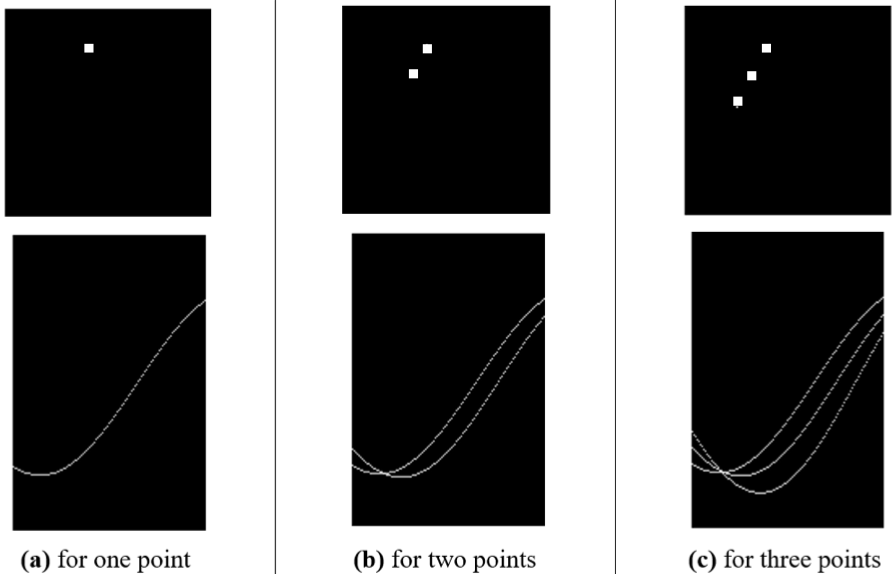
\includegraphics[scale=0.6]{Images/hough.png}
    \caption{Hough Space}
    \label{fig:hough}
\end{figure}

However, shapes are more complex than lines and sometimes cannot be defined by equations.

\subsection{Hough Transform for Complex Shapes}

Given a circle, we can find shapes (e.g. pupil) with the hugh transform. This is difficult in practice as most shapes are not exactly a circle. Again lets transform the equation to polar space.

\begin{align}
    (x-a)^{2} + (y-b)^{2} = r^{2} \\
    r = 2a\cos{\theta} + 2b\sin{\theta} \\
    \text{Where:} \\
    \text{r - radius of circle} \\
    \text{a - x coordinate of center} \\
    \text{b - y coordinate of center}
\end{align}

\noindent The same process of iteration can be applied, and the peaks used to determine points of interest.

\subsubsection{Addition: Elipse}

An elipse can be described mathematically:

\begin{equation}
    \frac{(x-x0)^{2}}{a^{2}}+\frac{(y-y0)^{2}}{b^{2}} = 1
\end{equation}

We can see that we have 4 separate parameters. If we have 100 values, and add rotation, we have a huge amount of values stored in accumulator space. This motivates approaches to save memory and improve speed.

\subsubsection{3D Accumulator}

Lets take the circle equation:

\begin{equation}
    (x-a)^{2} + (y-b)^{2} = r^{2} 
\end{equation}

We can differentiate the following equation, and substitute it back into the equation:

\begin{align}
    \frac{\delta y}{\delta x} = - \frac{(x-x_{0})}{(y-y_{0})} \\
    (\frac{\delta y}{\delta x})^{2}(y-y_{0})^{2}+(y-y_{0})^{2} = r^{2} \\
    y-y_{0} = \frac{r}{\sqrt{1+(\frac{\delta y}{\delta x})^{2}}}
\end{align}

\subsubsection{Arbitrary Shapes}
We use the generalised hough transform, form a discrete R table, and vote via the look up table. \\

\noindent We start from a reference point within the shape, and determine different edge vectors.